\chapter{Camera Geometry}
In this chapter we provide a basic background about image formation, camera geometry, multiview geometry and OpenGL notation. 
The system proposed in this thesis builds its principles and its implementation on these tools. 
We first, describe how the image project on a standard camera, by describing the classical pin-hole model and the transformations involved. 
Then we extend the discussion to the two or multiple view case, where more than one camera look at the scene. Multiple camera are needed to reconstruct the 3D structure of a general scene.
Finally, we describe how openGL represents image formation and we provide a connection with the standard pin-hole model.


\minitoc

\section{Image Formation}
The understanding of how the image has been generated is crucial in most computer vision applications. For instance to reconstruct the 3D geometry of the scene, a model that describes how the scene project on the images is needed. 
The classical approach to describe image formation, relies on the so called pin-hole camera model.
This model is a very effective compromise between mathematical simplicity and expressiveness.

Let assume that the world reference frame has its center $C$ in the camera center, the $Z$ axis along the principal axis of the camera, and the $Y$ and $X$ axis oriented upward and left-wise (Figure \ref{fig:pinhole}). 
We define $f$ as the focal length, that is the distance between the camera center and the image plane.
With basic geometry (see Figure \ref{fig:pinhole}(b)), the relation between  point $\mathbf{X} = \{X, Y, Z\}$ and $\mathbf{x}$ can be expressed as follows:
\begin{equation}
\label{eq:proj}
 \mathbf{x} = 
 \begin{pmatrix}
 fX/Z\\
 fY/Z\\
 f
 \end{pmatrix}
\end{equation}
The $x$ and $y$ coordinates of this point represent the position of $\mathbf{x}$ in the image plane, where the 2D reference frame is defined by the axis $x_{\text{cam}}$ and $y_{\text{cam}}$ which lay on the image plane and intersect the principal axis.
By representing $\mathbf{X}$ and $\mathbf{x}$ in homogeneous coordinates, Equation \ref{eq:proj} writes:
\begin{equation}
\label{eq:intrSimple}
 \mathbf{x}^{\text{cam}} = 
 \begin{pmatrix}
 x^{cam}\\
 y^{cam}\\
 1
 \end{pmatrix} =
 \begin{pmatrix}
 fX\\
 fY\\
 Z
 \end{pmatrix}=
 \begin{pmatrix}
 f&0&0&0\\
 0&f&0&0\\
 0&0&1&0
 \end{pmatrix} 
 \begin{pmatrix}
 X\\
 Y\\
 Z\\
 1
 \end{pmatrix}
\end{equation}

\begin{figure}[t]
 \begin{tabular}{cc}
  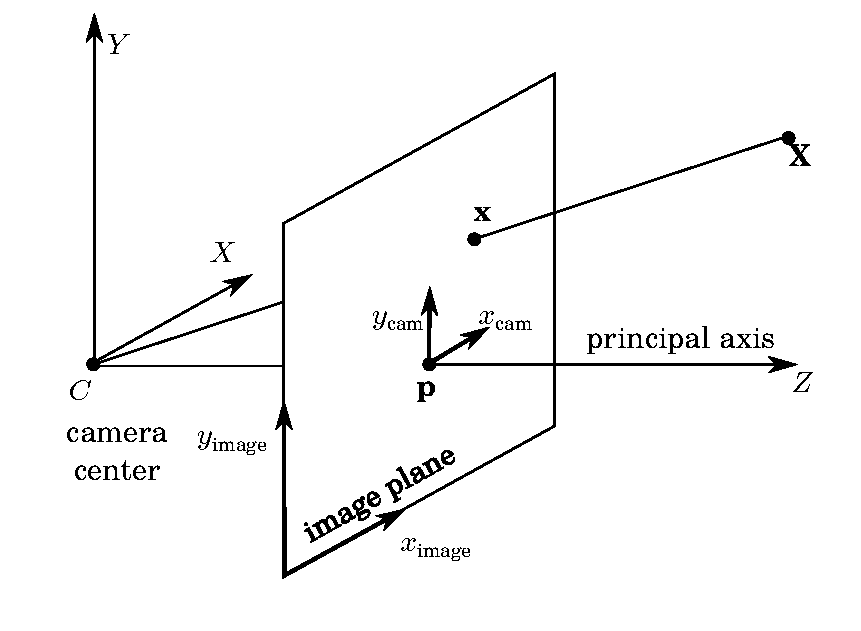
\includegraphics[width=0.48\columnwidth]{./img/ch-camera/camera}&
  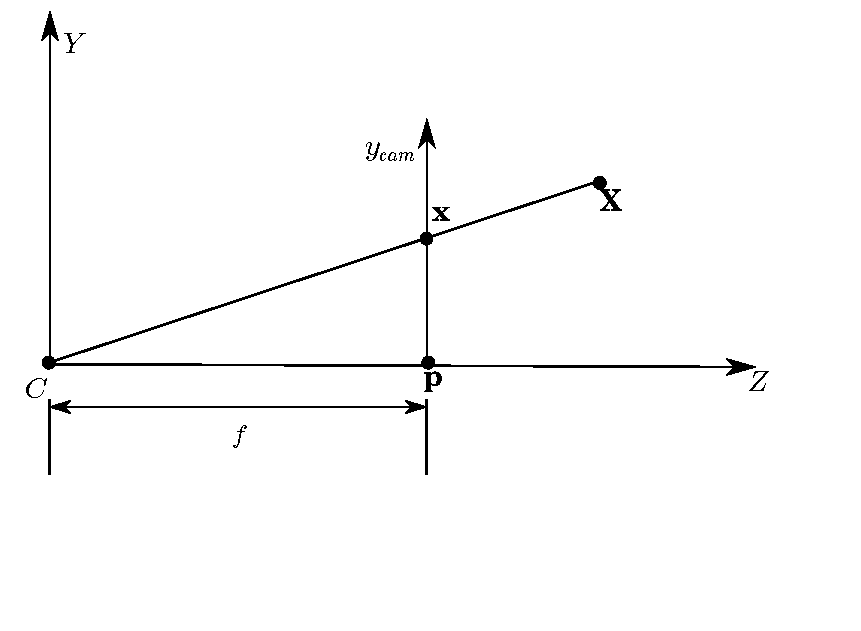
\includegraphics[width=0.48\columnwidth]{./img/ch-camera/camera01}\\
  (a)&(b)
 \end{tabular}
 \caption{Pin-hole camera.}
 \label{fig:pinhole}
\end{figure}
Since an image is represented with a matrix, the coordinates $(0,0)$ are not the center of it; therefore a more practical reference frame on the image plane can be defined as in Figure \ref{fig:centercamera}. Equation \eqref{eq:intrSimple} becomes:
\begin{equation}
\label{eq:intrCompl}
 \mathbf{x}^{\text{image}} = 
 \begin{pmatrix}
 x^{cam} + p_x\\
 y^{cam} + p_y\\
 1
 \end{pmatrix} =
 \begin{pmatrix}
 f&0&p_x&0\\
 0&f&p_y&0\\
 0&0&1&0
 \end{pmatrix} 
 \begin{pmatrix}
 X\\
 Y\\
 Z\\
 1
 \end{pmatrix}
\end{equation}.
The camera 
\begin{equation}
K = 
\begin{pmatrix}
 f&0&p_x\\
 0&f&p_y\\
 0&0&1
 \end{pmatrix} 
\end{equation}
is named \emph{intrinsic camera}, and $f$, $p_x$ and $p_y$ are the \emph{intrinsic parameters}. 

\begin{figure}[t]
  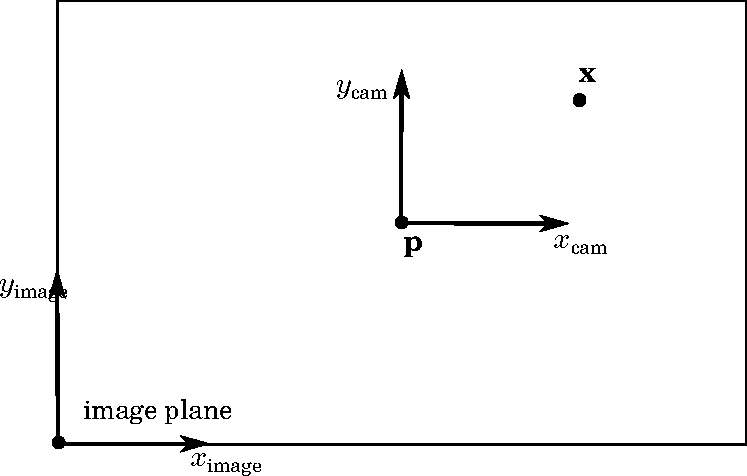
\includegraphics[width=0.8\columnwidth]{./img/ch-camera/camera02}\\
 \caption{Coordinates on the image plane.}
 \label{fig:centercamera}
\end{figure}
The assumption of a world reference frame coinciding with the camera frame is a very particular case. We now generalize the previous relation between a 3D point in the a generic world reference frame $\mathcal{W}$ and the 2D point in the image plane where the 3D point projects.
Let $C^\mathcal{W}$ be the center of the camera in the world reference $\mathcal{W}$ and  $R_\mathcal{C}^\mathcal{W}$ the rotation of the camera frame $\mathcal{C}$ with respect to $\mathcal{W}$: the matrix 
\begin{equation}
E_\mathcal{C}^\mathcal{W} = 
\begin{pmatrix}
R_\mathcal{C}^\mathcal{W} &C^\mathcal{W}\\
\mathbf{0}&1
 \end{pmatrix}   
\end{equation}
 describes the roto-translation of the camera with respect to the world reference frame.

The 3D point in Equation \ref{eq:intrCompl} is in the camera reference frame, but usually 3D points have to be expressed in the world coordinates. Therefore we rewrite the equation:


\begin{equation}
 \mathbf{x}^{\text{image}} =
\begin{pmatrix}
 K &\mathbf{0}
 \end{pmatrix} 
 \mathbf{X}^\mathcal{C}
 = 
\begin{pmatrix}
 K &\mathbf{0}
 \end{pmatrix} 
\begin{pmatrix}
 E_\mathcal{C}^\mathcal{W}
 \end{pmatrix}^{-1}
 \mathbf{X}^\mathcal{W}
\end{equation}
The matrix 
\begin{equation}
  E = (E_\mathcal{C}^\mathcal{W})ì{-1} = E_\mathcal{W}^\mathcal{C} = 
\begin{pmatrix}
R_\mathcal{W}^\mathcal{C} & - R_\mathcal{C}^\mathcal{W} C^\mathcal{W}\\
\mathbf{0}&1
 \end{pmatrix} 
\end{equation}
is usually referred as \emph{extrinsic matrix}: it is a roto-translation that transforms points in world coordinates to the camera reference frame.

In conclusion, the projection of a 3D point in the world to the image plane is computed as
\begin{equation}
 \mathbf{x}^{\text{image}}
 = 
\begin{pmatrix}
 K &\mathbf{0}
 \end{pmatrix} 
E
\:
 \mathbf{X}^\mathcal{W}\:=
P
\:
 \mathbf{X}^\mathcal{W}
\end{equation}
where matrix $P$ is the \emph{calibration matrix} which express both the parameters intrinsic to the specific camera (intrinsic matrix) and the position and orientation of the camera (extrinsic matrix).


\section{Multi-View Geometry}
In the reconstruction process two or more views are involved, indeed two or more 2D measurements are needed to disambiguate and estimate the 3D position. 
In this section we explain the basic principles underlying the geometry of two cameras in the projective space described thus far.
\subsection{Epipolar geometry}
The geometry between two views is known as \emph{epipolar geometry}: it depends only on the camera parameters, and is independent from the structure of the observed scene.
The epipolar geometry originates whenever two cameras look at the same scene. 
Let $C_1$ and $C_2$ be two cameras defined by the intrinsic matrices $K_1$ and $K_2$ and the extrinsic matrices $E_1$ and $E_2$.
A point $X$,  visible from both cameras, projects in the 2D point $x_1$ and $x_2$ of the $C_1$ and   $C_2$ image plane.
The camera centers $C_1$ and $C_2$, the points $x_1$ and $x_2$ and $X$ lays on the same plane $\pi$ (Figure \ref{fig:epipolar}) named \emph{epipolar plane}. 
If our information about $X$ is represented only by the projection $x_1$, we can deduce that the projection on $C_2$ of the corresponding 3D point is constrained to lay on the line, named \emph{epipolar line}, which is the projection of the viewing ray from $C_1$ to $x_1$.


\begin{figure}[t]
  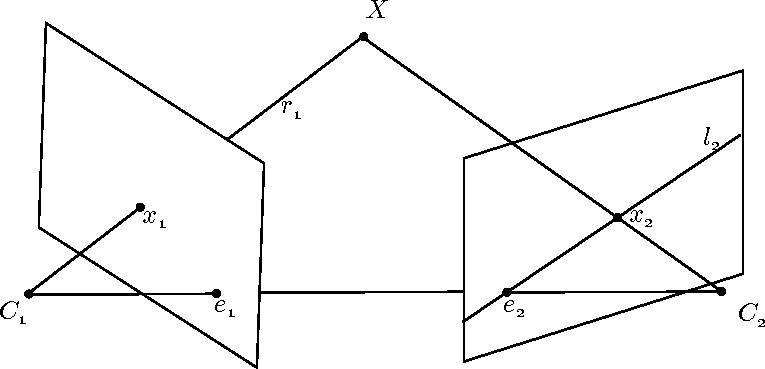
\includegraphics[width=0.8\columnwidth]{./img/ch-camera/cameraEpipolar}\\
 \caption{Two view: epipolar geometry.}
 \label{fig:epipolar}
\end{figure}


\subsection{Triangulation}
\subsection{Gauss-Newton for Position Refinement}
\section{OpenGL Camera}
